\documentclass[UTF8,fontset=none,aspectratio=169,10pt]{beamer}
\usepackage{ads-beamer-theme}

\title{高级分布式系统}
\subtitle{第八讲：容器编排与微服务}
\author{陈鹏飞\quad 计算机学院}
\institute{中山大学}
\date{2025--2026 学年}

\begin{document}

\begin{frame}[plain]
\begin{tikzpicture}[remember picture,overlay]
  \fill[ADSBlue] (current page.north west) rectangle ([xshift=2.4cm]current page.south west);
  \fill[ADSOrange] ([xshift=2.4cm]current page.north west) rectangle ([xshift=2.55cm]current page.south west);
  \node[anchor=west,align=left] at ([xshift=3.3cm,yshift=1.0cm]current page.west) {\fontsize{32}{38}\selectfont\color{ADSBlue}\bfseries 高级分布式系统};
  \node[anchor=west,align=left] at ([xshift=3.3cm,yshift=-0.4cm]current page.west) {\fontsize{21}{27}\selectfont\color{ADSDarkBlue}第八讲\quad 容器编排与微服务};
  \node[anchor=west,align=left] at ([xshift=3.3cm,yshift=-2.2cm]current page.west) {\large\color{ADSGray}从“把程序装进容器”走向“在故障不断的集群上持续运行应用”};
  \node[anchor=east] at ([xshift=-0.8cm,yshift=-3.2cm]current page.east) {\small\color{ADSGray}陈鹏飞\quad 中山大学\quad 2025--2026};
  \draw[ADSBlue,line width=0.8pt] ([xshift=3.3cm,yshift=-1.35cm]current page.west) -- ([xshift=12.6cm,yshift=-1.35cm]current page.west);
\end{tikzpicture}
\end{frame}

\sectionframe{一、先建立问题：为什么需要容器编排？}{从单机交付到集群运行，问题会依次变成环境、故障、调度、网络、存储、升级和隔离。}

\begin{frame}{本讲的学习目标}
\begin{enumerate}
  \item 解释容器与虚拟机的边界：它们分别隔离什么、共享什么；
  \item 从 Dockerfile、镜像仓库和运行时串起软件交付链；
  \item 读懂 Kubernetes 的控制面、节点、Pod 和 Service；
  \item 用“期望状态—观测状态—控制器动作”解释副本、升级和故障恢复；
  \item 把这些原语迁移到 GPU 训练、模型服务和 AI 集群。
\end{enumerate}
\vfill
\callout{听课抓手}{每个新对象都问三件事：它想隐藏什么复杂性？它靠什么状态做决定？失败时谁把系统拉回来？}
\end{frame}

\begin{frame}{一条贯穿全讲的因果链}
\begin{center}
\begin{tikzpicture}[node distance=8mm and 9mm,>=Latex]
  \nodebox[minimum width=2.45cm]{ADSOrange}{env}{环境漂移};
  \nodebox[right=of env,minimum width=2.45cm]{ADSBlue}{container}{容器封装};
  \nodebox[right=of container,minimum width=2.45cm]{ADSGreen}{cluster}{集群规模};
  \nodebox[below=of env,minimum width=2.45cm]{ADSOrange}{failure}{常态故障};
  \nodebox[right=of failure,minimum width=2.45cm]{ADSBlue}{control}{声明式控制};
  \nodebox[right=of control,minimum width=2.45cm]{ADSGreen}{ai}{AI 基础设施};
  \draw[\arrow,ADSGray] (env)--(container);
  \draw[\arrow,ADSGray] (container)--(cluster);
  \draw[\arrow,ADSGray] (cluster.south)--(failure.north);
  \draw[\arrow,ADSGray] (failure)--(control);
  \draw[\arrow,ADSGray] (control)--(ai);
\end{tikzpicture}
\end{center}
\vfill
\callout{核心转折}{容器解决“怎样打包并启动”；编排系统解决“在不断变化的资源和故障中，怎样持续满足目标”。}
\end{frame}

\begin{frame}{Google 的系统背景：规模先把“偶发故障”变成“日常事件”}
\begin{columns}[T]
\column{.52\linewidth}
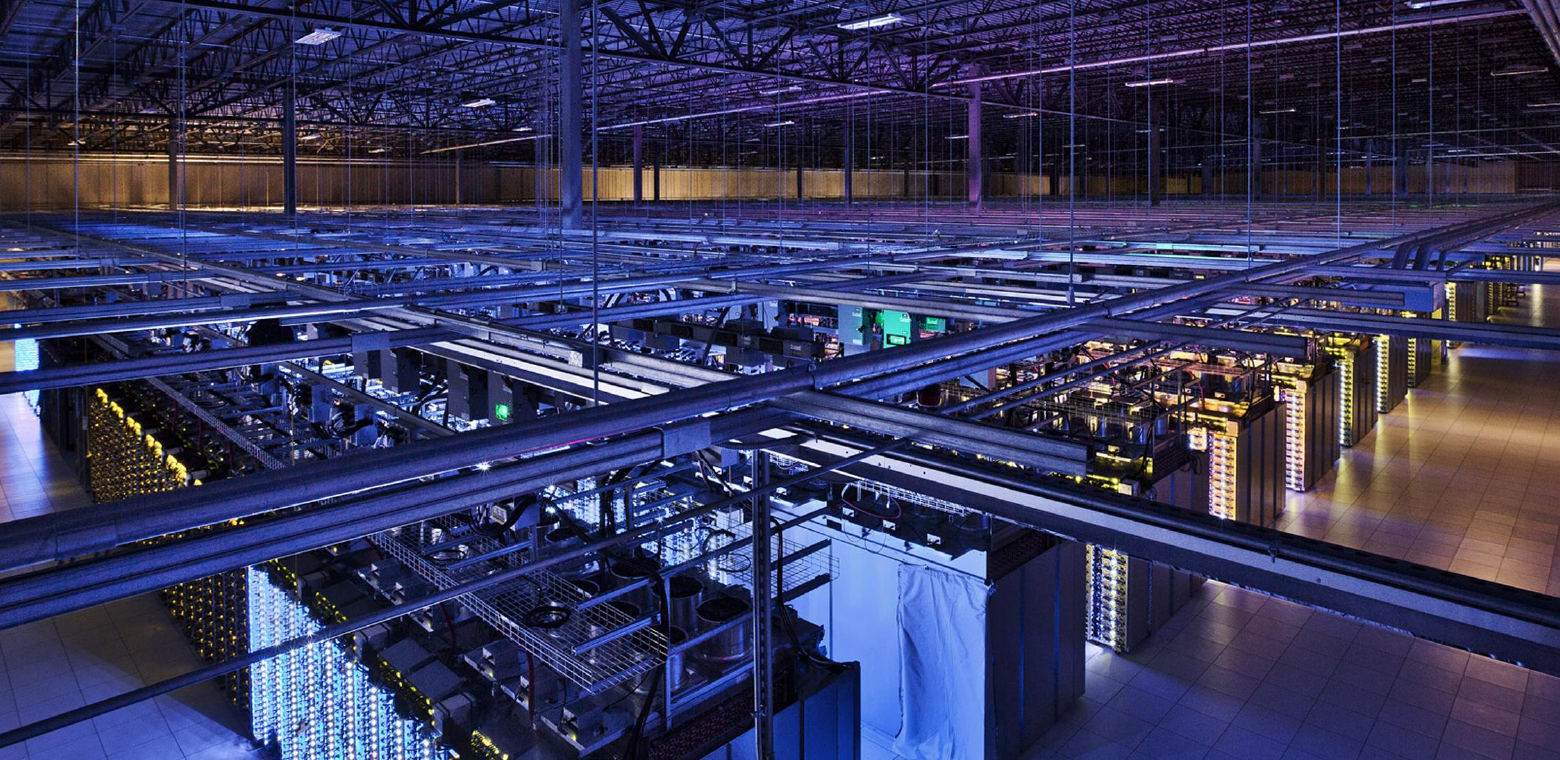
\includegraphics[width=\linewidth,height=.53\paperheight,keepaspectratio]{assets/week08-source-2025/datacenter.png}
\column{.44\linewidth}
\begin{itemize}
  \item 大型集群不是“很多台可靠机器”，而是大量独立故障源的组合；
  \item 在 2000 台机器的集群中，每天出现 1--10 台机器故障可以是正常现象；
  \item 因此应用不能把某台机器、某个 IP、某个进程 ID 当作永久事实；
  \item 编排层必须提供重新放置、重启、发现和流量切换。
\end{itemize}
\end{columns}
\smallnote{数据中心照片用来引出“失败是常态”的系统假设。}
\end{frame}

\begin{frame}{故障不是例外，而是编排系统的输入}
\begin{columns}[T]
\column{.52\linewidth}
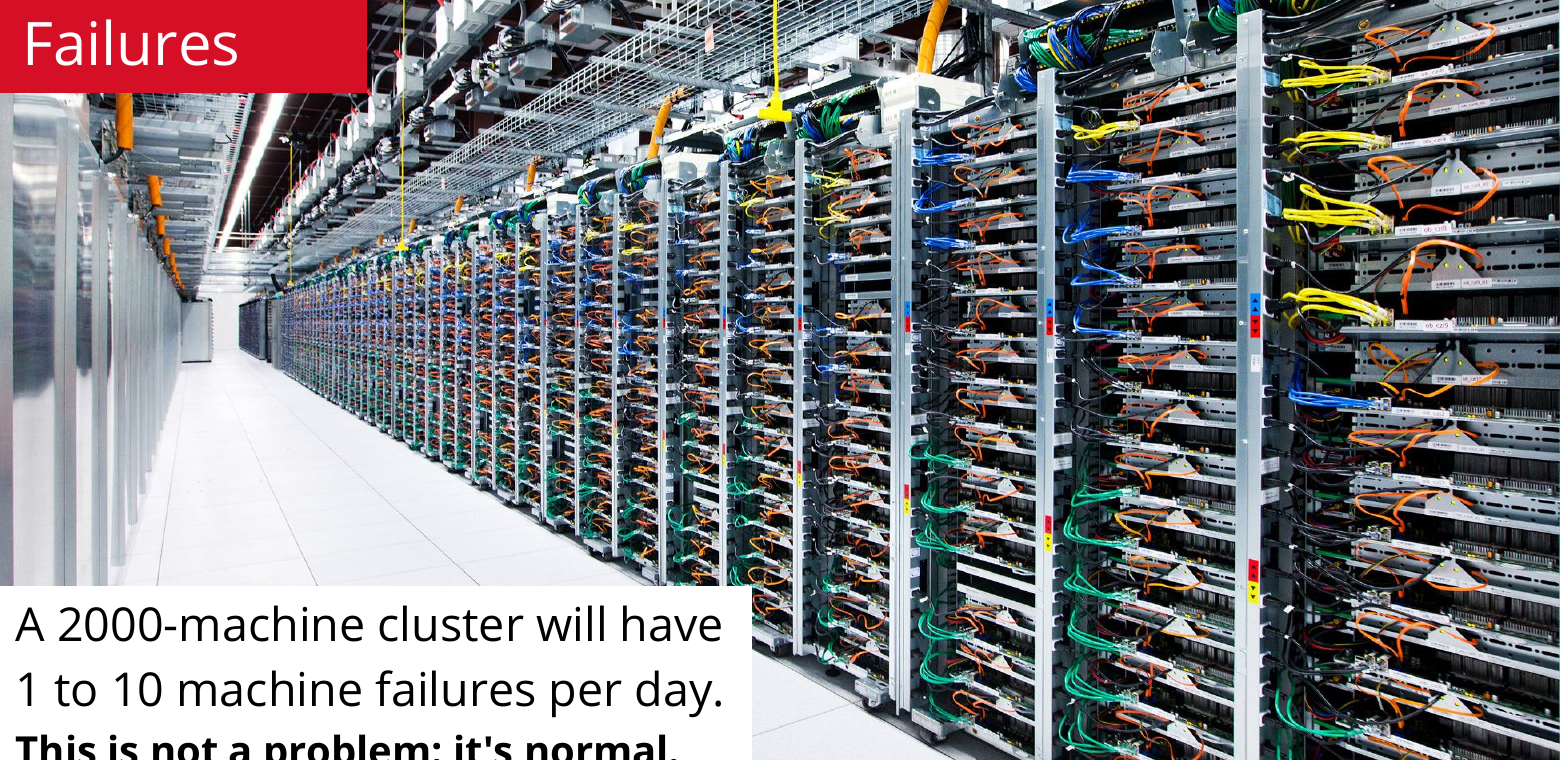
\includegraphics[width=\linewidth,height=.53\paperheight,keepaspectratio]{assets/week08-source-2025/failures-cluster.png}
\column{.44\linewidth}
\begin{itemize}
  \item 节点可能掉电、网络分区、磁盘损坏或内核失联；
  \item 容器可能崩溃、内存超限、探针失败或镜像拉取失败；
  \item 控制器看到的不是“故障原因”，而是实际状态与期望状态的差距；
  \item 学习 Kubernetes，首先要接受：恢复动作是持续发生的控制过程。
\end{itemize}
\end{columns}
\end{frame}

\begin{frame}{从开发者视角重新定义“机器”}
\begin{itemize}
  \item 传统部署：开发者选择机器、端口、目录和启动顺序；
  \item 集群部署：开发者提交应用描述，平台选择机器并负责生命周期；
  \item 机器变成可替换的资源池，应用身份由标签、服务名和持久化数据承载；
  \item 这不是“少写几条命令”，而是把控制权从命令序列转移到系统状态。
\end{itemize}
\vfill
\callout{问题}{如果一个 Pod 被删掉后，新 Pod 的 IP 和节点都变了，哪些信息必须保持不变，客户端才不会感知？}
\end{frame}

\sectionframe{二、容器：共享内核的进程封装}{容器的价值不是“更小的虚拟机”，而是用操作系统原语把进程、文件系统和资源边界组合起来。}

\begin{frame}{容器到底隔离了什么？}
\begin{columns}[T]
\column{.48\linewidth}
\begin{itemize}
  \item \textbf{Namespaces}：看到不同的进程、网络、挂载点和主机名；
  \item \textbf{cgroups}：限制 CPU、内存、块设备和 PID 等资源使用；
  \item \textbf{chroot / rootfs}：给进程一套独立的文件系统视图；
  \item 容器仍共享宿主机内核，因此启动快、密度高，但隔离边界不是虚拟机级别。
\end{itemize}
\column{.48\linewidth}
\resizebox{.98\linewidth}{!}{%
\begin{tikzpicture}[node distance=5mm and 7mm,>=Latex]
  \nodebox[minimum width=2.8cm,minimum height=.8cm]{ADSBlue}{host}{宿主机内核};
  \nodebox[below left=of host,minimum width=2.7cm]{ADSGreen}{c1}{容器 A\\namespace + cgroup};
  \nodebox[below right=of host,minimum width=2.7cm]{ADSOrange}{c2}{容器 B\\namespace + cgroup};
  \draw[\arrow,ADSGray] (host)--(c1);
  \draw[\arrow,ADSGray] (host)--(c2);
\end{tikzpicture}
}
\vfill
\smallnote{容器是“进程视图 + 资源边界 + 文件系统包”的组合。}
\end{columns}
\end{frame}

\begin{frame}{容器与虚拟机：隔离层次不同}
\begin{tabularx}{\linewidth}{>{\bfseries}p{2.7cm}XX}
\toprule
维度 & 容器 & 虚拟机 \\
\midrule
内核 & 与宿主机共享 & 每个虚机有客体内核 \\
启动 & 通常毫秒到秒级 & 通常秒到分钟级 \\
密度 & 高，适合微服务 & 低，边界更强 \\
故障边界 & 受宿主机内核影响 & 由虚拟化层切开 \\
适合场景 & 交付一致性、快速伸缩 & 强隔离、异构内核、传统系统 \\
\bottomrule
\end{tabularx}
\vfill
\callout{不要混淆}{容器提升的是交付和调度效率，不等于自动获得虚拟机的安全隔离。}
\end{frame}

\begin{frame}{容器的第二个价值：把依赖封装成可搬运的包}
\begin{itemize}
  \item 镜像是 hermetic bundle：程序、运行时、依赖和默认配置一起封装；
  \item “在我的电脑上能运行”被转化为“同一镜像在不同节点上执行”；
  \item 外部依赖仍要显式处理：数据库、密钥、对象存储、GPU 驱动和网络；
  \item 因而镜像解决的是软件供应链，Volume/Secret/Service 解决的是运行时依赖。
\end{itemize}
\vfill
\callout{课堂检查}{如果把数据库数据写进镜像层，容器删除后数据会怎样？为什么这不是镜像该负责的事情？}
\end{frame}

\begin{frame}{容器运行时的生命周期}
\begin{center}
\begin{tikzpicture}[node distance=8mm and 8mm,>=Latex]
  \nodebox{ADSBlue}{pull}{拉取镜像};
  \nodebox[right=of pull]{ADSOrange}{create}{创建 rootfs};
  \nodebox[right=of create]{ADSGreen}{isolate}{建立隔离};
  \nodebox[right=of isolate]{ADSBlue}{start}{启动进程};
  \nodebox[right=of start]{ADSOrange}{observe}{采集状态};
  \draw[\arrow,ADSGray] (pull)--(create);
  \draw[\arrow,ADSGray] (create)--(isolate);
  \draw[\arrow,ADSGray] (isolate)--(start);
  \draw[\arrow,ADSGray] (start)--(observe);
  \draw[\arrow,ADSGray] (observe) .. controls +(0,-1) and +(0,-1) .. (isolate);
\end{tikzpicture}
\end{center}
\begin{itemize}
  \item 运行时把“镜像内容”变成“节点上的进程”；
  \item Kubernetes 不直接替代运行时，而是通过 kubelet 调用运行时并管理更高层的生命周期。
\end{itemize}
\end{frame}

\begin{frame}{Dockerfile：从源代码到镜像层}
\scriptsize
\begin{block}{一个最小 Node.js 镜像}
\texttt{FROM node:18}\par
\texttt{WORKDIR /app}\par
\texttt{COPY package*.json ./}\par
\texttt{RUN npm ci --only=production}\par
\texttt{COPY server.js ./}\par
\texttt{CMD ["node", "server.js"]}
\end{block}
\begin{itemize}
  \item 每条指令通常形成一层；层可缓存、可复用、可按摘要寻址；
  \item 先复制依赖清单再安装，是为了让源代码改动不触发整层重建；
  \item 镜像构建是可重复的编译过程，而不是在服务器上手工安装软件。
\end{itemize}
\end{frame}

\begin{frame}{镜像构建：缓存、上下文与可复现性}
\begin{enumerate}
  \item 客户端把 build context 发送给构建器；
  \item 构建器按 Dockerfile 顺序解析每一步；
  \item 若指令与输入摘要未变，则复用缓存层；
  \item 最终得到 manifest + layer digests；
  \item 任何节点只要能按摘要拉到这些层，就能得到同一份文件系统。
\end{enumerate}
\vfill
\callout{工程陷阱}{把整个源码目录和密钥放进 build context，会导致镜像泄露、缓存失效和构建变慢；用 .dockerignore 明确边界。}
\end{frame}

\begin{frame}{构建与运行命令的含义}
\begin{tabularx}{\linewidth}{>{\ttfamily}p{4.2cm}X}
\toprule
命令 & 对分布式交付链的意义 \\
\midrule
docker build -t repo/app:v1 . & 把源码和 Dockerfile 编译为镜像 \\
docker run -p 8080:8080 repo/app:v1 & 在本机创建隔离进程，并做端口映射 \\
docker push repo/app:v1 & 把 manifest 与层上传到仓库 \\
docker pull repo/app:v1 & 在另一台机器按标签解析并下载镜像 \\
\bottomrule
\end{tabularx}
\vfill
\callout{重要}{标签是人类可读的别名；摘要才是内容寻址的稳定身份。生产发布应记录不可变 digest。}
\end{frame}

\begin{frame}{镜像仓库：让“同一软件”跨机器移动}
\begin{center}
\begin{tikzpicture}[node distance=8mm and 11mm,>=Latex]
  \nodebox[minimum width=2.5cm]{ADSOrange}{dev}{开发机};
  \nodebox[right=of dev,minimum width=2.7cm]{ADSBlue}{registry}{镜像仓库\\manifest + layers};
  \nodebox[right=of registry,minimum width=2.5cm]{ADSGreen}{node}{集群节点};
  \draw[\arrow,ADSGray] (dev)--node[above,font=\scriptsize]{push}(registry);
  \draw[\arrow,ADSGray] (registry)--node[above,font=\scriptsize]{pull}(node);
  \draw[->,ADSGray] (node.south) .. controls +(0,-.8) and +(0,-.8) .. node[below,font=\scriptsize]{digest 校验} (registry.south);
\end{tikzpicture}
\end{center}
\begin{itemize}
  \item 仓库把构建与运行解耦；节点不必拥有源码，只需拥有镜像；
  \item 失败恢复时，调度器可以把 Pod 放到另一台节点并重新拉取镜像；
  \item 这正是“不可变工件 + 可替换实例”的第一版实现。
\end{itemize}
\end{frame}

\begin{frame}{课堂互动：为什么本机成功、集群失败？}
\begin{enumerate}
  \item 本机用的是 ARM 镜像，集群节点是 x86；
  \item 镜像里写死了 localhost 数据库；
  \item 容器以非 root 用户运行，但目录权限不匹配；
  \item 镜像标签被覆盖，节点缓存了旧版本；
  \item 配置和密钥被写进了开发机环境变量，镜像并未携带。
\end{enumerate}
\vfill
\callout{讨论方式}{两人一组：先分类为“构建问题 / 运行时依赖 / 集群调度问题”，再说出一个可观测证据。}
\end{frame}

\sectionframe{三、Kubernetes：从启动容器到管理应用状态}{Kubernetes 的抽象不是“更复杂的 Docker 命令”，而是把集群当成一个可编程的控制系统。}

\begin{frame}{Kubernetes 的名字与目标}
\begin{itemize}
  \item Kubernetes 源自希腊语“舵手”，强调在变化环境中操纵系统；
  \item 它管理容器集群，但不要求应用知道具体云厂商或具体机器；
  \item 目标是管理应用，而不是让开发者逐台管理机器；
  \item API、调度器、控制器、节点代理和存储共同组成“云操作系统”的骨架。
\end{itemize}
\vfill
\callout{系统视角}{Kubernetes 不是一个单点服务，而是多个控制环围绕一个可观测 API 状态库协作。}
\end{frame}

\begin{frame}{Kubernetes 的 10000 英尺视图}
\begin{center}
\begin{tikzpicture}[>=Latex,node distance=7mm and 10mm,font=\small,scale=.84,transform shape]
  \nodebox[minimum width=2.0cm]{ADSOrange}{user}{用户 / 运维者};
  \nodebox[right=of user,minimum width=2.2cm]{ADSBlue}{api}{API Server};
  \nodebox[right=of api,minimum width=2.0cm]{ADSGreen}{etcd}{etcd 状态库};
  \nodebox[below=of api,xshift=-1.35cm,minimum width=2.2cm]{ADSBlue}{sched}{调度器};
  \nodebox[below=of api,xshift=1.35cm,minimum width=2.2cm]{ADSBlue}{ctrl}{控制器};
  \draw[\arrow,ADSGray] (user)--node[above,font=\scriptsize]{CLI / API / UI}(api);
  \draw[<->,ADSGray] (api)--(etcd);
  \draw[<->,ADSGray] (api)--(sched);
  \draw[<->,ADSGray] (api)--(ctrl);
  \node[draw=ADSGray!55,rounded corners,minimum width=10.7cm,minimum height=2.0cm,
        below=17mm of sched.south east,anchor=north east,label={[font=\small\bfseries]above left:工作节点（数据面）}] (nodes) {};
  \node[draw=ADSOrange!70!black,fill=ADSOrange!10,rounded corners=2pt,minimum width=2.1cm,minimum height=.62cm,align=center,font=\scriptsize]
    (k1) at ([xshift=-3.5cm]nodes.center) {节点代理 kubelet};
  \nodebox[right=7mm of k1,minimum width=2.1cm]{ADSGreen}{r1}{容器运行时};
  \nodebox[right=7mm of r1,minimum width=2.1cm]{ADSBlue}{p1}{Pod 实例};
  \nodebox[right=7mm of p1,minimum width=2.1cm]{ADSBlue}{p2}{Pod 实例};
  \draw[\arrow,ADSGray] (api.south) -- ++(0,-.45) -| node[pos=.78,left,font=\scriptsize]{对象与绑定结果}(k1.north);
  \draw[\arrow,ADSGray] (k1)--(r1);
  \draw[\arrow,ADSGray] (r1)--(p1);
  \draw[\arrow,ADSGray] (r1.south) .. controls +(0,-.35) and +(0,-.35) .. (p2.south);
\end{tikzpicture}
\end{center}
\smallnote{所有声明先进入 API Server；调度器和控制器通过 watch 推动状态收敛，kubelet 只负责本节点上的实际执行。}
\end{frame}

\begin{frame}{控制面与数据面：职责必须分开}
\begin{tabularx}{\linewidth}{>{\bfseries}p{2.8cm}XX}
\toprule
组件 & 主要职责 & 学生应记住的状态 \\
\midrule
API Server & 认证、校验、读写对象、提供 watch & 所有声明的入口 \\
etcd & 持久化一致的集群状态 & 期望状态与对象元数据 \\
Scheduler & 为未绑定 Pod 选择节点 & 资源、约束、拓扑 \\
Controller & 观察差距并发起动作 & 期望状态与实际状态 \\
Kubelet & 在节点执行 Pod 生命周期 & 节点上的实际状态 \\
\bottomrule
\end{tabularx}
\vfill
\callout{关键边界}{控制面决定“应该在哪里、应该有几个”；kubelet 负责“在这台机器上把它跑起来”。}
\end{frame}

\begin{frame}{一次 kubectl apply 究竟发生了什么？}
\begin{enumerate}
  \item 用户提交 YAML；
  \item API Server 做认证、准入和 schema 校验；
  \item 对象写入 etcd，成为新的期望状态；
  \item Controller watch 到对象变化，创建或更新下游对象；
  \item Scheduler 为尚未绑定的 Pod 选择节点；
  \item kubelet watch 到绑定结果，调用运行时拉镜像并启动容器；
  \item 状态沿 kubelet $\rightarrow$ API Server $\rightarrow$ etcd 回写，用户通过 watch 看到收敛过程。
\end{enumerate}
\end{frame}

\begin{frame}{声明式与命令式：差别在于谁持有“真相”}
\begin{columns}[T]
\column{.48\linewidth}
\blocktitle{命令式}
\begin{itemize}
  \item 依次执行“创建、启动、扩容、重启”；
  \item 顺序和当前环境耦合；
  \item 中途失败后，下一次执行要猜测已经完成了什么。
\end{itemize}
\column{.48\linewidth}
\blocktitle{声明式}
\begin{itemize}
  \item 只提交“我要 4 个副本”；
  \item 控制器反复比较实际状态；
  \item 重试是安全的，控制环最终把系统拉回目标。
\end{itemize}
\end{columns}
\vfill
\callout{一句话}{命令式脚本描述路径；声明式配置描述终点。分布式系统更需要描述终点。}
\end{frame}

\begin{frame}{创建集群：难但不可避免的那一半}
\begin{enumerate}
  \item 选择云、裸金属或本地环境；
  \item 选择节点操作系统和容器运行时；
  \item 供应机器，安装控制面和节点组件；
  \item 规划 Pod、Service、节点和外部网络地址段；
  \item 启动 DNS、日志、监控和证书等基础服务；
  \item 管理内核升级、硬件故障和节点生命周期。
\end{enumerate}
\vfill
\callout{为什么需要托管服务}{集群搭建是基础设施工程；托管 Kubernetes 把这部分复杂性外包，让开发者把时间放在应用对象上。}
\end{frame}

\begin{frame}{使用集群：应用开发者真正关心的部分}
\begin{itemize}
  \item 创建 Pod、ReplicaSet、Deployment、DaemonSet 和 StatefulSet；
  \item 暴露 Service，挂载 Volume，注入 Secret 与 ConfigMap；
  \item 使用探针、自动扩缩容、日志、监控和调试工具；
  \item 这些对象共同描述“应用应该怎样存活、怎样被访问、怎样升级”。
\end{itemize}
\vfill
\callout{抽象边界}{开发者不应被迫处理每台节点的 IP、网卡和进程号；平台把这些变化压缩成稳定 API。}
\end{frame}

\begin{frame}{工作负载可移植性：write once, run anywhere？}
\begin{itemize}
  \item 应用只依赖 Kubernetes API，而不是某个云厂商专属脚本；
  \item Pod 网络、Service、Ingress、PersistentVolume 等抽象隐藏底层实现；
  \item 同一份应用描述可以在本地、云上和裸金属之间迁移；
  \item 但“可移植”不是“零差异”：性能、GPU 驱动、存储类别和网络 SLA 仍需要适配。
\end{itemize}
\vfill
\callout{现实主义}{Kubernetes 降低的是控制面锁定，不会消除所有硬件和云服务差异。}
\end{frame}

\begin{frame}{从“应用知道云”到“平台提供能力”}
\begin{tabularx}{\linewidth}{>{\bfseries}p{3.2cm}XX}
\toprule
能力 & 不可移植写法 & Kubernetes 风格 \\
\midrule
网络入口 & 写死云厂商负载均衡 IP & Service / Ingress \\
持久化 & 直接调用某云块存储 SDK & PersistentVolumeClaim \\
配置 & 把配置打进镜像 & ConfigMap \\
凭证 & 把密钥放进代码或镜像 & Secret + 外部密钥系统 \\
伸缩 & 自己调用云 API & HPA / Cluster Autoscaler \\
\bottomrule
\end{tabularx}
\end{frame}

\sectionframe{四、网络：容器为什么需要重新定义“地址”}{从 Docker 的端口映射，到 Kubernetes 的 Pod IP 和 Service 名称，网络抽象逐步把客户端与实例解耦。}

\begin{frame}{Docker 默认网络：私有地址 + NAT}
\begin{center}
\begin{tikzpicture}[node distance=9mm and 10mm,>=Latex]
  \nodebox[minimum width=2.4cm]{ADSBlue}{client}{客户端};
  \nodebox[right=of client,minimum width=2.8cm]{ADSOrange}{host}{宿主机\\192.168.1.10:8080};
  \nodebox[right=of host,minimum width=2.8cm]{ADSGreen}{container}{容器\\172.17.0.2:80};
  \draw[\arrow,ADSGray] (client)--node[above,font=\scriptsize]{端口映射}(host);
  \draw[\arrow,ADSGray] (host)--node[above,font=\scriptsize]{NAT}(container);
\end{tikzpicture}
\end{center}
\begin{itemize}
  \item 容器地址通常是宿主机私有网络的一部分；
  \item 对外访问需要端口映射，多个容器容易产生端口冲突；
  \item 这对单机开发足够，但对跨节点服务发现不够。
\end{itemize}
\end{frame}

\begin{frame}{端口映射解决了可达性，却没有解决身份}
\begin{itemize}
  \item 客户端需要知道宿主机地址和映射端口；
  \item 容器重启后，端口可能变、节点可能变；
  \item 多个副本需要负载均衡，故障副本必须自动摘除；
  \item 因此 Kubernetes 把“实例 IP”与“服务身份”分离：Pod 可变，Service 稳定。
\end{itemize}
\vfill
\callout{类比}{Pod 像电话号码会变化的员工；Service 像公司的总机号码，负责找到当前可用员工。}
\end{frame}

\begin{frame}{Kubernetes 网络模型}
\begin{itemize}
  \item 每个 Pod 获得一个集群范围内的 IP；
  \item Pod 之间可以直接通信，即使位于不同节点；
  \item 不要求应用自己做端口经纪和节点级 NAT；
  \item 底层可以是三层路由、云网络或覆盖网络，但 Pod 看到的是统一地址空间；
  \item 这一模型让应用连接的是逻辑对端，而不是节点上的随机端口。
\end{itemize}
\vfill
\callout{代价}{统一地址空间需要网络插件、路由规则和故障探测；“简单的应用网络”把复杂性推给了平台。}
\end{frame}

\begin{frame}{Pod 网络的跨节点路径}
\begin{center}
\begin{tikzpicture}[node distance=8mm and 12mm,>=Latex]
  \nodebox[minimum width=2.5cm]{ADSBlue}{p1}{Pod A\\10.2.1.4};
  \nodebox[right=of p1,minimum width=2.5cm]{ADSDarkBlue}{n1}{Node 1\\CNI 路由};
  \nodebox[right=of n1,minimum width=2.5cm]{ADSDarkBlue}{n2}{Node 2\\CNI 路由};
  \nodebox[right=of n2,minimum width=2.5cm]{ADSGreen}{p2}{Pod B\\10.2.3.7};
  \draw[\arrow,ADSGray] (p1)--(n1);
  \draw[\arrow,ADSGray] (n1)--node[above,font=\scriptsize]{underlay / overlay}(n2);
  \draw[\arrow,ADSGray] (n2)--(p2);
\end{tikzpicture}
\end{center}
\begin{itemize}
  \item 网络插件负责把 Pod CIDR 与节点网络连接起来；
  \item 应用只需要目标 Pod IP 或 Service 名称，不需要知道具体隧道。
\end{itemize}
\end{frame}

\begin{frame}{课堂互动：从客户端到 Pod 的路由链}
\begin{enumerate}
  \item 客户端访问 \texttt{api.default.svc.cluster.local:80}；
  \item DNS 返回 Service 的虚拟 IP；
  \item kube-proxy / eBPF 规则把虚拟 IP 选择到某个后端 Pod；
  \item CNI 将数据包送到目标节点的 Pod 网卡；
  \item Pod 内部进程监听容器端口并返回响应。
\end{enumerate}
\vfill
\callout{追问}{如果一个后端 Pod 变成 NotReady，哪一层应该把它从可选后端集合中移除？为什么不能依赖客户端自己重试？}
\end{frame}

\sectionframe{五、Pod：调度与协作的最小单位}{Pod 把需要一起放置、一起启动、共享网络和卷的容器绑定成一个生命周期。}

\begin{frame}{为什么 Kubernetes 不直接调度单个容器？}
\begin{itemize}
  \item 有些容器必须共享 localhost、IPC、卷或生命周期；
  \item 例如数据拉取器和 Web 服务：一个准备内容，一个对外提供内容；
  \item 若分别调度，二者可能分到不同节点，通信和数据共享都要重新设计；
  \item Pod 把这类强耦合容器作为一个原子放置单元。
\end{itemize}
\vfill
\callout{调度原子性}{调度器先决定“这个 Pod 去哪”，再由 kubelet 在该节点启动其中的多个容器。}
\end{frame}

\begin{frame}{Pod 的共享语义}
\begin{columns}[T]
\column{.46\linewidth}
\begin{itemize}
  \item 共享一个 Pod IP 和网络命名空间；
  \item 容器可以用 localhost 互访；
  \item 可以挂载同一个 Volume；
  \item 共享生命周期，但容器仍有各自的进程和资源限制。
\end{itemize}
\column{.50\linewidth}
\begin{center}
\begin{tikzpicture}[font=\small,>=Latex]
  \node[draw=ADSBlue,rounded corners,minimum width=5.6cm,minimum height=4.5cm,
        label={[font=\small\bfseries]above:同一个 Pod}] (pod) {};
  \node[draw=ADSBlue!70!black,fill=ADSBlue!10,rounded corners=2pt,minimum width=2.0cm,minimum height=.62cm,align=center,font=\scriptsize]
    (puller) at ([xshift=-1.25cm,yshift=.75cm]pod.center) {文件拉取容器};
  \node[draw=ADSOrange!70!black,fill=ADSOrange!10,rounded corners=2pt,minimum width=2.0cm,minimum height=.62cm,align=center,font=\scriptsize]
    (web) at ([xshift=1.25cm,yshift=.75cm]pod.center) {Web 服务容器};
  \node[draw=ADSGreen!70!black,fill=ADSGreen!10,rounded corners=2pt,minimum width=3.0cm,minimum height=.62cm,align=center,font=\scriptsize]
    (vol) at ([yshift=-1.15cm]pod.center) {共享卷 Volume};
  \draw[\arrow,ADSGray] (puller.south)--(vol.north west);
  \draw[\arrow,ADSGray] (vol.north east)--(web.south);
  \node[font=\scriptsize,text=ADSGray] at ([yshift=1.65cm]pod.center) {共享 Pod IP、localhost 与生命周期};
\end{tikzpicture}
\end{center}
\end{columns}
\smallnote{文件拉取容器把内容写入共享卷，Web 容器从同一卷读取；二者必须被调度到同一节点并共同重建。}
\end{frame}

\begin{frame}{Pod 是可替换实例，不是永久身份}
\begin{itemize}
  \item Pod 绑定到一个节点；节点故障后，原 Pod 不会“带着同一个 ID 复活”；
  \item 新 Pod 会得到新的 UID、IP 和运行时状态；
  \item 应用需要稳定身份时，应使用 Service、StatefulSet 或外部存储；
  \item 这就是“实例可变、服务稳定、数据持久”的分层。
\end{itemize}
\vfill
\callout{设计判断}{如果业务逻辑依赖 Pod 名称或 IP，通常说明应用把平台的临时身份误当成了业务身份。}
\end{frame}

\begin{frame}{Volume：把生命周期从容器中分离出来}
\begin{itemize}
  \item EmptyDir：Pod 生命周期内的临时共享目录；
  \item HostPath：直接使用节点目录，简单但可移植性和隔离性较弱；
  \item 网络文件系统、云块存储、分布式文件系统：把数据生命周期交给外部系统；
  \item Secret、ConfigMap 也通过 Volume 形式注入文件，但语义不是通用持久化。
\end{itemize}
\vfill
\callout{核心问题}{容器重启后，什么数据必须保留？谁拥有这些数据？答案决定 Volume 类型。}
\end{frame}

\begin{frame}{Labels：给对象附加可查询的元数据}
\begin{itemize}
  \item Label 是键值对，可附着在 Pod、Node、Service、Deployment 等 API 对象上；
  \item 它通常表达身份：\texttt{app=payments}、\texttt{version=v2}、\texttt{zone=az1}；
  \item 其他控制器通过 Selector 查询标签，而不是维护一份静态对象清单；
  \item 标签是弱耦合的连接点：发布、服务发现、调度约束都可复用同一套元数据。
\end{itemize}
\end{frame}

\begin{frame}{Selectors：Kubernetes 中的“集合连接器”}
\begin{center}
\begin{tikzpicture}[node distance=7mm and 10mm,>=Latex]
  \nodebox[minimum width=2.5cm]{ADSBlue}{pods}{Pod 集合};
  \nodebox[right=of pods,minimum width=2.8cm]{ADSOrange}{selector}{selector: app=web};
  \nodebox[right=of selector,minimum width=2.5cm]{ADSGreen}{service}{Service};
  \nodebox[below=of selector,minimum width=2.8cm]{ADSDarkBlue}{rs}{ReplicaSet};
  \draw[\arrow,ADSGray] (selector)--(service);
  \draw[\arrow,ADSGray] (selector)--(rs);
  \draw[<-,ADSGray] (pods)--(selector);
\end{tikzpicture}
\end{center}
\begin{itemize}
  \item Service 通过 selector 找后端；ReplicaSet 通过 selector 找自己管理的 Pod；
  \item 标签错误会造成“服务无后端”或“两个控制器争抢同一批 Pod”；
  \item 因而 selector 是配置中最需要做一致性检查的字段之一。
\end{itemize}
\end{frame}

\begin{frame}{Selector 的逐步收缩：从大集合到精确角色}
\scriptsize
\begin{tabularx}{\linewidth}{>{\bfseries}p{3.4cm}X}
\toprule
过滤条件 & 选中的对象 \\
\midrule
\texttt{app=MyApp} & 所有环境、所有版本、所有角色 \\
\texttt{app=MyApp, role=FE} & 只选前端角色 \\
\texttt{app=MyApp, phase=prod} & 只选生产对象 \\
\texttt{app=MyApp, phase=prod, role=FE} & 精确到生产前端 \\
\bottomrule
\end{tabularx}
\vfill
\callout{课堂练习}{给一个包含 v1/v2、prod/test、FE/BE 的四象限标签表，让学生预测三个不同 selector 的匹配集合。}
\end{frame}

\sectionframe{六、副本与控制环：让应用在故障后回到目标}{ReplicaSet 把“我要 N 个副本”变成持续运行的反馈控制问题。}

\begin{frame}{ReplicaSet 的唯一任务}
\begin{columns}[T]
\column{.48\linewidth}
\begin{itemize}
  \item 运行在 API Server 之外；
  \item 通过 selector 找到属于自己的 Pod；
  \item 数量少于目标：创建 Pod；
  \item 数量多于目标：删除多余 Pod；
  \item 不承诺副本顺序或永久身份。
\end{itemize}
\column{.48\linewidth}
\begin{center}
\begin{tikzpicture}[font=\small,>=Latex,node distance=8mm]
  \nodebox[minimum width=3.1cm]{ADSBlue}{desired}{期望副本数：4};
  \nodebox[below=of desired,minimum width=3.1cm]{ADSOrange}{observe}{实际 Ready Pod：3};
  \nodebox[below=of observe,minimum width=3.1cm]{ADSGreen}{action}{差值为 $+1$：创建 Pod};
  \draw[\arrow,ADSGray] (desired)--node[right,font=\scriptsize]{比较}(observe);
  \draw[\arrow,ADSGray] (observe)--(action);
  \draw[->,ADSGray] (action.west) .. controls +(-1.0,0) and +(-1.0,0) .. node[left,font=\scriptsize]{再次 watch}(observe.west);
\end{tikzpicture}
\end{center}
\end{columns}
\smallnote{控制器没有“完成”这一刻：每次对象变化、Pod 退出或节点失联，都会触发下一轮观测与调节。}
\end{frame}

\begin{frame}{把 ReplicaSet 写成一个控制环}
\begin{center}
\begin{tikzpicture}[node distance=10mm and 13mm,>=Latex]
  \nodebox[minimum width=2.5cm]{ADSBlue}{desired}{期望：replicas=4};
  \nodebox[right=of desired,minimum width=2.5cm]{ADSOrange}{observe}{观测：现有 Pod=3};
  \nodebox[right=of observe,minimum width=2.5cm]{ADSGreen}{act}{动作：创建 1 个};
  \draw[\arrow,ADSGray] (desired)--(observe);
  \draw[\arrow,ADSGray] (observe)--(act);
  \draw[->,ADSGray] (act.south) .. controls +(0,-1) and +(0,-1) .. node[below,font=\scriptsize]{下一次观测}(observe.south);
\end{tikzpicture}
\end{center}
\vfill
\begin{itemize}
  \item 控制器不需要知道上一次做过什么，只需反复计算差距；
  \item 这让重试、崩溃恢复和多控制器协作更容易推理。
\end{itemize}
\end{frame}

\begin{frame}{节点故障时，副本如何恢复？}
\begin{enumerate}
  \item Node 1 失联，原 Pod 状态逐渐被标记为 Unknown/Failed；
  \item ReplicaSet 看到可用副本数低于目标；
  \item Scheduler 为新 Pod 选择 Node 2；
  \item kubelet 拉取镜像、启动容器、执行探针；
  \item Service 只把 Ready 的新 Pod 加入后端。
\end{enumerate}
\vfill
\callout{重要}{“副本恢复”与“流量恢复”是两个控制环：前者创建实例，后者根据健康状态更新路由。}
\end{frame}

\begin{frame}{为什么 Deployment 要包住 ReplicaSet？}
\begin{itemize}
  \item ReplicaSet 擅长维持同一模板的副本数；
  \item 发布新版本时，需要同时管理旧 ReplicaSet 与新 ReplicaSet；
  \item Deployment 记录版本、升级策略、暂停/恢复和回滚；
  \item 旧 RS 不立即删除，因为回滚需要保留可用的历史模板。
\end{itemize}
\vfill
\callout{抽象层次}{Pod 解决“一个实例怎么跑”；ReplicaSet 解决“有多少实例”；Deployment 解决“版本怎样变化”。}
\end{frame}

\sectionframe{七、Service：把流量接到一组可替换 Pod}{Service 不是一个进程，而是一条稳定的访问策略：选择后端、分配虚拟地址并处理健康变化。}

\begin{frame}{Service 的语义}
\begin{itemize}
  \item Service 通过 selector 选择一组 Pod；
  \item 为这组 Pod 提供稳定的虚拟 IP、端口和 DNS 名称；
  \item 后端 Pod 可以被替换，客户端不必重新发现实例；
  \item Service 还隐含访问策略：谁能访问、流量如何分配、是否暴露到集群外。
\end{itemize}
\vfill
\callout{状态变化}{Pod 集合是动态的，Service 的 Endpoints/EndpointSlices 是控制器根据标签和 Ready 状态计算出来的。}
\end{frame}

\begin{frame}{Service 的数据路径}
\begin{center}
\begin{tikzpicture}[node distance=8mm and 12mm,>=Latex]
  \nodebox[minimum width=2.4cm]{ADSBlue}{client2}{客户端};
  \nodebox[right=of client2,minimum width=2.8cm]{ADSOrange}{vip}{Service VIP\\10.96.0.10:80};
  \nodebox[right=of vip,minimum width=2.4cm]{ADSGreen}{p1b}{Pod 1};
  \nodebox[below=of p1b,minimum width=2.4cm]{ADSGreen}{p2b}{Pod 2};
  \draw[\arrow,ADSGray] (client2)--(vip);
  \draw[\arrow,ADSGray] (vip)--(p1b);
  \draw[\arrow,ADSGray] (vip)--(p2b);
\end{tikzpicture}
\end{center}
\begin{itemize}
  \item VIP 是逻辑地址，后端 Pod IP 是实例地址；
  \item kube-proxy、iptables、IPVS 或 eBPF 负责把逻辑规则落实到数据路径。
\end{itemize}
\end{frame}

\begin{frame}{kube-proxy / iptables 的控制面到数据面}
\begin{enumerate}
  \item Service 对象写入 API Server；
  \item EndpointSlice 控制器根据 selector 生成后端集合；
  \item kube-proxy watch 到变化，编程节点上的 iptables/IPVS 规则；
  \item 数据包到达 Service VIP 后，在节点内选择后端 Pod；
  \item 后端失败或 NotReady 时，规则集合更新，停止向它转发。
\end{enumerate}
\vfill
\callout{讲授重点}{控制面更新规则不是每个请求都访问 API Server；数据面必须本地、快速、可缓存。}
\end{frame}

\begin{frame}{Service 完整过程（上）：控制面生成后端集合}
\begin{enumerate}
  \item[$t_0$] 用户提交 Service 与 Pod/Deployment 对象。API Server 持久化的是“期望状态”，它本身不转发业务流量。
  \item[$t_1$] Pod 被调度、启动并接受 Readiness 检查。只有 Ready 实例才应进入可服务集合，避免请求过早到达。
  \item[$t_2$] EndpointSlice 控制器把 selector 与 Pod 标签匹配，写入 Pod IP、端口和 Ready 条件。
  \item[$t_3$] 各节点的 kube-proxy 或 eBPF agent 通过 watch 获得新版本，将其编译为本地 iptables、IPVS 或 eBPF 规则。
\end{enumerate}
\vfill
\callout{为什么分层}{Service 表达稳定身份，EndpointSlice 表达当前后端，节点规则落实快速转发。控制面对象和数据面规则职责不同，因此可以独立演进。}
\end{frame}

\begin{frame}{Service 完整过程（下）：一次请求如何到达 Pod}
\begin{enumerate}
  \item[$t_4$] 客户端通过 DNS 得到 Service 的 ClusterIP，并向 \texttt{ClusterIP:port} 发包；客户端不保存会变化的 Pod IP。
  \item[$t_5$] 数据包命中本节点的 Service 规则；规则只从 Ready Endpoint 中选择一个 Pod。
  \item[$t_6$] 数据面执行 DNAT、IPVS 调度或 eBPF 重定向，将目标改写/路由到具体 Pod IP。
  \item[$t_7$] Pod 返回响应；具体返回路径取决于 CNI、转发模式和是否发生 SNAT。
\end{enumerate}
\vfill
\callout{关键区分}{Service/EndpointSlice 属于控制面状态；iptables、IPVS 或 eBPF 映射属于数据面状态。两者短暂不同步时，系统依赖 watch、资源版本和重复协调最终收敛。}
\end{frame}

\begin{frame}{Service 后端失败：摘除过程不是瞬时完成}
\begin{center}
\begin{tikzpicture}[node distance=8mm and 10mm,>=Latex]
  \nodebox[minimum width=2.2cm]{ADSGreen}{healthy}{Pod Ready};
  \nodebox[right=of healthy,minimum width=2.2cm]{ADSOrange}{probe}{探针失败};
  \nodebox[right=of probe,minimum width=2.5cm]{ADSBlue}{ep}{EndpointSlice\\Ready=false};
  \nodebox[right=of ep,minimum width=2.5cm]{ADSGray}{rules}{节点规则更新};
  \draw[\arrow,ADSGray] (healthy)--node[above]{周期检测}(probe);
  \draw[\arrow,ADSGray] (probe)--node[above]{状态上报}(ep);
  \draw[\arrow,ADSGray] (ep)--node[above]{watch}(rules);
\end{tikzpicture}
\end{center}
\begin{enumerate}
  \item 故障发生到探针判定之间仍可能有请求到达该 Pod；
  \item EndpointSlice 更新到所有节点规则收敛也需要时间；
  \item 因而客户端仍需设置超时、有限重试和幂等语义，不能把 Service 当成“零失败”抽象；
  \item 若重试没有退避或预算，多个客户端可能在摘除窗口形成重试风暴。
\end{enumerate}
\callout{例子}{探针周期 5 秒、失败阈值 3 次时，仅故障判定就可能接近 15 秒；这段时间决定了用户可见错误和尾延迟。}
\end{frame}

\begin{frame}{Service 类型：从集群内部到外部世界}
\begin{tabularx}{\linewidth}{>{\bfseries}p{2.8cm}XX}
\toprule
类型 & 地址范围 & 典型用途 \\
\midrule
ClusterIP & 集群内部虚拟 IP & 微服务之间调用 \\
NodePort & 每个节点开放端口 & 简单地从外部进入集群 \\
LoadBalancer & 云/硬件负载均衡器 & 对外提供稳定入口 \\
ExternalName & DNS 别名 & 把外部服务纳入发现体系 \\
\bottomrule
\end{tabularx}
\vfill
\callout{设计选择}{内部调用优先使用 ClusterIP；对外暴露要考虑 TLS、认证、限流、健康检查和成本。}
\end{frame}

\begin{frame}{外部访问：LoadBalancer 与 Ingress 分工不同}
\begin{columns}[T,onlytextwidth]
\column{.47\textwidth}
\blocktitle{Service / LoadBalancer（主要是 L4）}
\begin{itemize}
  \item 按 IP、TCP/UDP 端口暴露一个 Service；
  \item 云控制器通常申请外部负载均衡器；
  \item 每个 Service 单独暴露时，地址和负载均衡器成本可能较高；
  \item 适合非 HTTP 协议或需要独立地址的服务。
\end{itemize}
\column{.47\textwidth}
\blocktitle{Ingress / Gateway（L7）}
\begin{itemize}
  \item 根据域名、URL path、Header 等把请求路由到不同 Service；
  \item 可集中终止 TLS、配置证书和 HTTP 重定向；
  \item API 对象只是声明，必须由 Ingress/Gateway controller 落实数据面；
  \item 适合多个 Web 服务共享入口。
\end{itemize}
\end{columns}
\vfill
\callout{请求链}{客户端 $\rightarrow$ 外部负载均衡器 $\rightarrow$ Ingress/Gateway 数据面 $\rightarrow$ ClusterIP Service $\rightarrow$ Ready Pod。每一跳都有独立的健康检查和收敛延迟。}
\end{frame}

\begin{frame}{Service 与应用协议：端口不是全部}
\begin{itemize}
  \item HTTP/HTTPS、gRPC、WebSocket 都需要稳定的逻辑入口；
  \item Service 只负责连接与转发，不理解业务重试、幂等和事务；
  \item 连接池、超时、熔断、重试等应由客户端库或服务网格补充；
  \item 如果只增加副本而不控制重试，故障时可能放大流量。
\end{itemize}
\vfill
\callout{分布式系统提醒}{服务发现解决“找到谁”，不保证“对方一定成功”；可靠性仍需要端到端协议。}
\end{frame}

\begin{frame}{课堂互动：Service 为什么没有后端？}
\begin{enumerate}
  \item Service selector 写成 \texttt{app=web}，Pod 标签写成 \texttt{app=frontend}；
  \item Pod 处于 Running 但 Readiness 探针失败；
  \item Service 与 Pod 位于不同 Namespace；
  \item targetPort 与容器实际监听端口不一致；
  \item NetworkPolicy 或节点路由阻断了数据面。
\end{enumerate}
\vfill
\callout{回答要求}{不能只说“网络有问题”，要指出对象状态、标签集合和数据路径中的具体证据。}
\end{frame}

\sectionframe{八、滚动升级：让版本变化也成为控制环}{升级不是“一次替换所有实例”，而是在可用性、速度和回滚之间管理两组副本。}

\begin{frame}{Rolling Update 的目标}
\begin{itemize}
  \item 新版本逐步增加，旧版本逐步减少；
  \item Service 在迁移过程中持续有 Ready 后端；
  \item 版本变化可暂停、可观察、可回滚；
  \item 更新动作不能依赖固定 Pod 身份，因为 Pod 是可替换的。
\end{itemize}
\vfill
\callout{不变量}{在升级窗口内，至少保持规定数量的可用副本；升级速度不能突破容量和安全约束。}
\end{frame}

\begin{frame}{Rolling Update 的一个快照}
\begin{center}
\begin{tikzpicture}[font=\small,>=Latex,node distance=7mm and 9mm]
  \nodebox[minimum width=2.8cm]{ADSBlue}{service}{稳定入口 Service};
  \nodebox[below left=of service,minimum width=3.0cm]{ADSGray}{oldrs}{旧副本集：版本 v1};
  \nodebox[below right=of service,minimum width=3.0cm]{ADSGreen}{newrs}{新副本集：版本 v2};
  \draw[\arrow,ADSGray] (service)--node[left,font=\scriptsize]{仍接收流量}(oldrs);
  \draw[\arrow,ADSGreen] (service)--node[right,font=\scriptsize]{Ready 后加入}(newrs);
  \foreach \x in {-1.0,0,1.0}{
    \node[draw=ADSGray,rounded corners,fill=ADSGray!8,minimum width=.78cm,minimum height=.55cm]
      at ([xshift=\x cm,yshift=-1.0cm]oldrs.south) {v1};
  }
  \foreach \x in {-.55,.55}{
    \node[draw=ADSGreen,rounded corners,fill=ADSGreen!8,minimum width=.78cm,minimum height=.55cm]
      at ([xshift=\x cm,yshift=-1.0cm]newrs.south) {v2};
  }
  \node[font=\scriptsize,text=ADSOrange] at ([yshift=-1.75cm]service.south) {扩新 $\rightarrow$ 就绪检查 $\rightarrow$ 摘除并缩旧};
\end{tikzpicture}
\end{center}
\smallnote{旧、新副本集在迁移窗口内同时存在；Service 只选择满足标签且通过就绪检查的 Pod。}
\end{frame}

\begin{frame}{Rolling Update 完整例子：6 个副本如何逐批替换}
\footnotesize
设 $replicas=6$、$maxSurge=2$、$maxUnavailable=1$。表中“后端”只统计 Ready Pod。
\begin{tabularx}{\linewidth}{>{\bfseries}p{1.2cm}*{4}{>{\centering\arraybackslash}X}}
\toprule
阶段 & 旧 Pod & 新 Pod & Ready 后端 & 运行总数 \\
\midrule
$s_0$ & 6 & 0 & 6 & 6 \\
$s_1$ & 6 & 2 & 6 & 8 \\
$s_2$ & 6 & 2 & 8 & 8 \\
$s_3$ & 4 & 2 & 6 & 6 \\
$s_4$ & 4 & 4 & 6--8 & 8 \\
$s_5$ & 2 & 4 & 6 & 6 \\
$s_6$ & 0 & 6 & 6 & 6 \\
\bottomrule
\end{tabularx}
\begin{itemize}
  \item $s_1$：先利用 surge 额度创建 2 个新 Pod；未 Ready 前不进入 Service。
  \item $s_3$：新 Pod Ready 后，旧 Pod 先摘除流量、排空连接，再终止。
  \item $s_4$--$s_6$：重复“扩新—验证—缩旧”，直到新 ReplicaSet 达到 6。
\end{itemize}
\smallnote{若某批新 Pod 一直不 Ready，Deployment 不应继续删除旧 Pod；这正是 maxUnavailable 与 Readiness 共同保护可用性的原因。}
\end{frame}

\begin{frame}{Rolling Update 的三条状态线}
\begin{center}
\begin{tikzpicture}[x=1.35cm,y=.8cm,>=Latex]
  \draw[->,ADSGray] (0,0)--(7.2,0) node[right]{阶段};
  \foreach \x/\lab in {0/$s_0$,1/$s_1$,2/$s_2$,3/$s_3$,4/$s_4$,5/$s_5$,6/$s_6$}
    \draw (\x,0.08)--(\x,-0.08) node[below]{\lab};
  \draw[very thick,ADSBlue] plot coordinates {(0,3.0)(1,3.0)(2,3.0)(3,2.0)(4,2.0)(5,1.0)(6,0)};
  \draw[very thick,ADSGreen] plot coordinates {(0,0)(1,1.0)(2,1.0)(3,1.0)(4,2.0)(5,2.0)(6,3.0)};
  \draw[very thick,ADSOrange,dashed] plot coordinates {(0,3.0)(1,3.0)(2,4.0)(3,3.0)(4,3.0)(5,3.0)(6,3.0)};
  \node[ADSBlue,anchor=west] at (6.35,0.2){旧副本};
  \node[ADSGreen,anchor=west] at (6.35,3.1){新副本};
  \node[ADSOrange,anchor=west] at (6.35,2.2){Ready 后端};
  \node[rotate=90,anchor=south] at (-.45,2.0){相对数量};
\end{tikzpicture}
\end{center}
\begin{itemize}
  \item 旧副本递减和新副本递增并非严格同步，中间由探针结果形成停顿；
  \item Service 看到的是 Ready 后端线，而不是“已创建 Pod”线；
  \item 发布系统的核心不是把版本号改掉，而是在约束下维护可用容量不变量。
\end{itemize}
\end{frame}

\begin{frame}{maxUnavailable 与 maxSurge}
\begin{tabularx}{\linewidth}{>{\bfseries}p{3.1cm}XX}
\toprule
参数 & 约束 & 直觉 \\
\midrule
maxUnavailable & 升级期间最多允许多少副本不可用 & 控制风险、保护容量 \\
maxSurge & 超过期望副本数最多临时增加多少副本 & 换取速度、消耗额外资源 \\
\bottomrule
\end{tabularx}
\vfill
\begin{itemize}
  \item 例如期望副本数为 6、maxUnavailable=1、maxSurge=2；
  \item 控制器可以先创建 2 个新 Pod，再等待 Ready，然后删除旧 Pod；
  \item 实际可行性还受节点资源、镜像拉取、探针和拓扑约束影响。
\end{itemize}
\end{frame}

\begin{frame}{升级失败：为什么要有暂停和回滚？}
\begin{enumerate}
  \item 新版本 Pod 反复 CrashLoopBackOff；
  \item Ready 数量上不去，Deployment 的进度条件超时；
  \item 控制器暂停继续扩大新版本；
  \item 运维检查日志、指标和错误率；
  \item 回滚到上一版本 ReplicaSet，恢复服务；
  \item 修复镜像或配置后，再次启动升级。
\end{enumerate}
\vfill
\callout{可靠性原则}{发布系统必须把“变化”当作可观测、可逆、可限速的状态转换。}
\end{frame}

\begin{frame}{滚动升级中的服务流量}
\begin{itemize}
  \item Pod 启动完成不代表可以接收流量；
  \item Readiness Probe 决定是否进入 Service 后端集合；
  \item PreStop、terminationGracePeriod 与连接排空避免请求被突然截断；
  \item 版本标签要同时服务于 selector、监控聚合和回滚定位；
  \item 对有状态系统，还需考虑分片迁移、主从角色和数据兼容。
\end{itemize}
\end{frame}

\sectionframe{九、工作负载类型：一次性、每节点与有状态}{不同工作负载的生命周期不同：不要用“永远运行的 Deployment”替代所有抽象。}

\begin{frame}{DaemonSet：每个节点都要有一个副本}
\begin{itemize}
  \item 典型对象：日志采集器、节点监控、网络插件、GPU 驱动代理；
  \item 新节点加入时自动创建 Pod；节点离开时一起删除；
  \item 可用 nodeSelector、亲和性和污点容忍限制节点子集；
  \item 它不是“副本数等于节点数”的手工脚本，而是节点集合上的控制环。
\end{itemize}
\vfill
\callout{AI 映射}{GPU 节点上的 device plugin、拓扑采集器和 NCCL 网络探针通常适合 DaemonSet。}
\end{frame}

\begin{frame}{Job：运行到完成，而不是永远服务}
\begin{itemize}
  \item Job 关注成功完成次数，而不是长期副本数；
  \item \texttt{parallelism} 表示并行运行上限；\texttt{completions} 表示需要成功完成多少个任务；
  \item Pod 失败时可按重试策略重建；
  \item 适合批处理、迁移、数据预处理和离线评估。
\end{itemize}
\vfill
\callout{AI 映射}{数据清洗、分片评测、Checkpoint 转换和离线 embedding 生成都是 Job/Workflow 的候选。}
\end{frame}

\begin{frame}{工作流：把多个 Job 连接起来}
\begin{center}
\begin{tikzpicture}[node distance=8mm and 12mm,>=Latex]
  \nodebox[minimum width=2.4cm]{ADSBlue}{prepare}{准备数据};
  \nodebox[right=of prepare,minimum width=2.4cm]{ADSOrange}{train}{训练/微调};
  \nodebox[right=of train,minimum width=2.4cm]{ADSGreen}{eval}{评测};
  \nodebox[right=of eval,minimum width=2.4cm]{ADSDarkBlue}{publish}{发布模型};
  \draw[\arrow,ADSGray] (prepare)--(train);
  \draw[\arrow,ADSGray] (train)--(eval);
  \draw[\arrow,ADSGray] (eval)--(publish);
\end{tikzpicture}
\end{center}
\begin{itemize}
  \item 每个阶段有自己的资源、失败策略和输出；
  \item 工作流控制器把“完成事件”转化为下游 Job 的期望状态；
  \item 这与分布式系统中的事件驱动协调、重试和幂等直接相关。
\end{itemize}
\end{frame}

\begin{frame}{PersistentVolume：把存储能力抽象出来}
\begin{itemize}
  \item 管理员提供存储资源，用户通过 PVC 声明需求；
  \item Pod 不直接绑定云厂商磁盘 ID；
  \item StorageClass 可以按性能、可用区和回收策略选择后端；
  \item 存储对象的生命周期可独立于 Pod，支持重启、迁移和回滚。
\end{itemize}
\vfill
\callout{关键分工}{管理员提供容量与策略；用户声明“我需要多大、什么访问模式、什么性能”。}
\end{frame}

\begin{frame}{PV/PVC/Pod 的绑定流程}
\begin{center}
\begin{tikzpicture}[font=\small,>=Latex,node distance=10mm and 12mm]
  \nodebox[minimum width=2.5cm]{ADSOrange}{admin}{管理员 / 动态供应器};
  \nodebox[right=of admin,minimum width=2.3cm]{ADSGreen}{pv}{持久卷 PV};
  \nodebox[below=of admin,minimum width=2.5cm]{ADSBlue}{user}{应用用户};
  \nodebox[right=of user,minimum width=2.3cm]{ADSBlue}{pvc}{存储声明 PVC};
  \nodebox[right=17mm of pv.south east,anchor=west,minimum width=2.5cm]{ADSOrange}{binder}{绑定控制器};
  \nodebox[right=of pvc,minimum width=2.5cm]{ADSGreen}{pod}{Pod 挂载卷};
  \draw[\arrow,ADSGray] (admin)--node[above,font=\scriptsize]{提供容量}(pv);
  \draw[\arrow,ADSGray] (user)--node[below,font=\scriptsize]{声明需求}(pvc);
  \draw[\arrow,ADSGray] (pv)--node[above,font=\scriptsize]{容量、模式、StorageClass}(binder);
  \draw[\arrow,ADSGray] (pvc)--node[below,font=\scriptsize]{请求条件}(binder);
  \draw[\arrow,ADSGreen] (binder)--node[right,font=\scriptsize]{绑定后可引用}(pod);
\end{tikzpicture}
\end{center}
\smallnote{PV 表示集群可提供的存储能力，PVC 表示应用需求；控制器匹配二者后，Pod 只引用 PVC，不直接绑定底层磁盘。}
\end{frame}

\begin{frame}{PV/PVC 的四个状态转换}
\begin{enumerate}
  \item Available：PV 尚未被声明；
  \item Bound：PVC 与 PV 匹配并锁定；
  \item Released：PVC 删除后，PV 释放但可能残留数据；
  \item Reclaimed：按回收策略保留、清理或重新提供。
\end{enumerate}
\vfill
\callout{数据安全}{删除 PVC 不等于删除业务数据；是否清理由 reclaimPolicy、快照和外部存储系统共同决定。}
\end{frame}

\begin{frame}{AI 训练中的存储分层}
\begin{tabularx}{\linewidth}{>{\bfseries}p{3.2cm}XX}
\toprule
层次 & 内容 & 典型接口 \\
\midrule
对象存储 & 原始数据、模型权重、归档 Checkpoint & S3 / OSS / GCS \\
共享文件系统 & 多 Pod 读取数据集、共享 tokenizer & NFS / CephFS / Lustre \\
本地 NVMe & 热数据、shuffle、编译缓存 & Local PV / EmptyDir \\
内存/显存缓存 & batch、KV cache、激活值 & Pod 本地进程 \\
\bottomrule
\end{tabularx}
\vfill
\callout{设计原则}{越靠近计算，延迟越低但故障后越容易丢失；Checkpoint 把可恢复性从节点本地提升到外部存储。}
\end{frame}

\sectionframe{十、配置、密钥与有状态工作负载}{镜像负责“软件是什么”，配置负责“这次怎样运行”，状态负责“过去发生了什么”。}

\begin{frame}{StatefulSet：当身份与顺序有意义}
\begin{itemize}
  \item StatefulSet 为副本提供稳定、可预测的名称和序号；
  \item 每个实例可以拥有独立的 PVC；
  \item 创建、删除和滚动更新可以按序进行；
  \item 适合数据库、ZooKeeper、Redis 集群等需要稳定身份的系统；
  \item 但 StatefulSet 不会自动解决数据库复制、选主和一致性协议。
\end{itemize}
\vfill
\callout{边界}{Kubernetes 管理进程与存储声明；应用自身仍需实现数据一致性、成员变更和故障恢复。}
\end{frame}

\begin{frame}{Deployment 与 StatefulSet 的对比}
\begin{tabularx}{\linewidth}{>{\bfseries}p{3cm}XX}
\toprule
属性 & Deployment & StatefulSet \\
\midrule
实例身份 & 可替换、无序 & 稳定名称和序号 \\
存储 & 通常共享或无状态 & 每个副本可有独立 PVC \\
更新 & 追求可用副本快速滚动 & 需要顺序和角色意识 \\
典型应用 & Web、API、无状态 worker & 数据库、队列、协调服务 \\
\bottomrule
\end{tabularx}
\end{frame}

\begin{frame}{ConfigMap：配置与镜像解耦}
\begin{itemize}
  \item 把环境、端口、特性开关和非敏感参数作为对象管理；
  \item 可以通过环境变量或 Volume 注入 Pod；
  \item 更新配置时，要明确应用是否会热加载；
  \item 配置对象也需要版本化，否则“同一个镜像”可能在不同环境表现不同。
\end{itemize}
\vfill
\callout{反模式}{把所有配置烘焙进镜像，会让环境差异变成镜像分叉，升级和回滚都更困难。}
\end{frame}

\begin{frame}{Secret：不要把秘密放进镜像}
\begin{itemize}
  \item Secret 用于密钥、令牌、证书和密码等敏感材料；
  \item 通过 API 权限、Namespace、外部 KMS 和审计控制谁能读取；
  \item Base64 编码不是加密，etcd 加密、密钥轮换和最小权限才是安全边界；
  \item 训练任务中的对象存储凭证、模型仓库 token、TLS 证书都应走 Secret/外部密钥系统。
\end{itemize}
\end{frame}

\begin{frame}{HPA：根据负载调整 Pod 数量}
\begin{itemize}
  \item Horizontal Pod Autoscaler 周期性读取 CPU、内存或自定义指标；
  \item 当观测值高于目标，增加副本；低于目标，减少副本；
  \item 有冷却、稳定窗口和最小/最大副本，避免抖动；
  \item HPA 只改变 Pod 数量，不保证节点资源足够，必要时还需 Cluster Autoscaler。
\end{itemize}
\vfill
\callout{控制理论}{HPA 是带滞后、采样周期和限幅的反馈控制器；指标延迟会直接影响扩缩容稳定性。}
\end{frame}

\begin{frame}{AI 推理中的自动扩缩容}
\begin{itemize}
  \item CPU 利用率可能不代表模型服务压力，队列长度、tokens/s、P99 延迟更合适；
  \item 扩容不仅要启动 Pod，还要拉取大模型、加载权重、预热 GPU；
  \item 缩容要处理会话、KV cache 和正在生成的请求；
  \item 因而 AI 服务常用“队列驱动 + 预测式扩容 + 预热池”组合，而不是只看 CPU。
\end{itemize}
\end{frame}

\sectionframe{十一、多租户与资源治理}{当多个团队共享集群，调度问题会变成公平性、隔离性、容量和优先级问题。}

\begin{frame}{Namespace：给对象划分逻辑空间}
\begin{itemize}
  \item Namespace 避免对象名称冲突，便于团队、环境和项目分区；
  \item RBAC、ResourceQuota、NetworkPolicy 等策略可按 Namespace 作用；
  \item Namespace 不是硬隔离：节点、内核、网络和存储仍可能共享；
  \item 多集群、多租户系统往往需要 Namespace + 节点池 + 身份系统的组合。
\end{itemize}
\vfill
\callout{命名层次}{同名的 Service 可以存在于不同 Namespace，但完整 DNS 名称必须包含 Namespace。}
\end{frame}

\begin{frame}{资源隔离：避免 noisy neighbor}
\begin{itemize}
  \item 一个工作负载过度消耗 CPU、内存、磁盘或网络，会影响其他应用；
  \item Kubernetes 通过 request/limit、cgroup、优先级和驱逐策略建立边界；
  \item 隔离既是性能问题，也是可用性和成本分摊问题；
  \item 对 GPU，显存、SM、NVLink 拓扑和 MIG 分区也要纳入资源模型。
\end{itemize}
\end{frame}

\begin{frame}{Request 与 Limit：两种不同承诺}
\begin{tabularx}{\linewidth}{>{\bfseries}p{2.8cm}XX}
\toprule
字段 & 对调度器的意义 & 对运行时的意义 \\
\midrule
Request & “我至少需要这么多”，用于放置和容量估计 & 影响资源保证和权重 \\
Limit & “最多允许用这么多” & 超出时节流、OOMKill 或驱逐 \\
\bottomrule
\end{tabularx}
\vfill
\begin{itemize}
  \item request 写得过小：调度器过度装箱，运行时争抢严重；
  \item limit 写得过小：应用频繁被杀；写得过大：集群可调度容量被虚占；
  \item 正确值需要来自压测、尾延迟和故障预算，而不是拍脑袋。
\end{itemize}
\end{frame}

\begin{frame}{Kubernetes QoS：由 request/limit 推导驱逐优先级}
\begin{tabularx}{\linewidth}{>{\bfseries}p{2.6cm}X X}
\toprule
QoS 类别 & 判定条件 & 节点资源紧张时的含义 \\
\midrule
Guaranteed & 每个容器都设置 CPU/内存 request 与 limit，且二者相等 & 保护最强，但仍可能因超过内存 limit 被 OOMKill \\
Burstable & 至少一个容器设置 request/limit，但不满足 Guaranteed & 可利用空闲资源，压力下按使用量和 request 关系驱逐 \\
BestEffort & 所有容器均未设置 CPU/内存 request/limit & 保护最低，通常最先被驱逐 \\
\bottomrule
\end{tabularx}
\vfill
\callout{不要误解}{QoS 是节点压力下的相对保护，不是端到端 SLA；网络、磁盘、GPU 和应用尾延迟仍需独立治理。}
\end{frame}

\begin{frame}{Quota 与 LimitRange：把资源治理放在入口}
\begin{itemize}
  \item ResourceQuota 限制一个 Namespace 的总 CPU、内存、Pod 数、PVC 数等；
  \item LimitRange 为单个容器提供默认 request/limit 和上下界；
  \item Admission Control 在对象写入前拒绝违规配置；
  \item 配额让“每个团队都申请无限资源”变成可审计、可预测的容量计划。
\end{itemize}
\vfill
\callout{AI 场景}{GPU 配额、优先级和抢占策略决定训练作业能否公平共享昂贵的加速器。}
\end{frame}

\begin{frame}{节点选择：标签、亲和性、污点与容忍}
\begin{itemize}
  \item nodeSelector：最简单的标签匹配；
  \item affinity/anti-affinity：表达“靠近/远离哪些工作负载”；
  \item taint：节点主动拒绝普通 Pod；toleration：Pod 明确声明可以进入；
  \item 这些机制共同表达硬件、故障域、合规和性能拓扑。
\end{itemize}
\vfill
\callout{AI 映射}{GPU 节点打 taint；训练 Pod 带 toleration，并用 node label 选择 A100/H100、NVLink 或特定可用区。}
\end{frame}

\begin{frame}{多可用区集群：副本数不等于故障域冗余}
\begin{itemize}
  \item 节点与持久卷通常带有 zone/region 标签；调度器必须让副本跨故障域分散。
  \item topology spread constraints 或 anti-affinity 可避免多个副本落在同一可用区。
  \item 区域故障时，控制面需要判断哪些 Pod 可重建、哪些 PVC 只能在原区挂载。
  \item Service 仍提供同一逻辑入口，但跨区流量会增加时延和费用。
  \item 对训练任务，跨区 GPU 通信通常代价过高；容灾副本与同步计算副本要分开设计。
\end{itemize}
\vfill
\callout{例子}{三个 Web 副本若都在 Zone A，replicas=3 仍无法抵抗 Zone A 故障；应把“数量约束”升级为“拓扑约束”。}
\end{frame}

\begin{frame}{Gang Scheduling：AI 训练的“要么一起到位”}
\begin{itemize}
  \item 数据并行/张量并行作业通常需要一组 GPU 同时就绪；
  \item 只启动部分 worker 会造成空转、超时和通信失败；
  \item Gang scheduler 先为整个作业预留一组资源，再同时放置 worker；
  \item 这与普通 Deployment 的“一个 Pod 一个 Pod 地扩展”不同。
\end{itemize}
\vfill
\callout{联系本讲}{Pod 是放置原子，但 AI 作业的调度原子可能是“PodGroup/JobGroup”；抽象层次要匹配应用的同步关系。}
\end{frame}

\begin{frame}{近期案例：Kueue/Volcano 类 GPU 队列调度}
\begin{itemize}
  \item 在线服务和训练作业共享 GPU 时，单个 Pod 的局部调度不足以表达“整组 worker 同时获得资源”；
  \item 队列系统通常把作业放入 queue，依据配额、优先级、资源 flavor 和抢占规则决定 admission；
  \item gang scheduling 把“部分启动、长期等待”改成“资源足够时整组准入”，减少分布式训练的假死；
  \item 控制器仍采用声明式 reconcile：准入记录、Pod 状态和租约可能暂时不一致，最终回到同一目标状态。
\end{itemize}
\vfill
\callout{课堂问题}{如果一个 8 卡作业只拿到 7 张卡，应该继续占位、回滚 admission，还是让出资源？请分别说明吞吐、公平和尾延迟后果。}
\end{frame}

\sectionframe{十二、伸缩与可扩展性：控制面也会成为瓶颈}{节点、Pod 和 API 调用数量增长后，编排系统自身必须有容量模型和分层控制。}

\begin{frame}{Cluster Autoscaler：什么时候增加节点？}
\begin{itemize}
  \item 集群中存在 Pending Pod；
  \item 评估增加某类节点后，是否能让至少一个 Pending Pod 获得可行放置；
  \item 若可行，扩容节点池；若长期空闲，则缩容节点；
  \item 受配额、云供应、启动时间、拓扑和 PodDisruptionBudget 约束。
\end{itemize}
\vfill
\callout{两层控制}{HPA 改变 Pod 数量；Cluster Autoscaler 改变节点数量。两者时间常数不同，容易出现“Pod 先扩、节点后到”的暂态。}
\end{frame}

\begin{frame}{AI 集群扩容的现实延迟}
\begin{enumerate}
  \item API 对象创建：秒级；
  \item 节点供应与启动：分钟级；
  \item GPU 驱动、网络插件和 device plugin 就绪：分钟级；
  \item 镜像和模型权重拉取：从秒到十几分钟；
  \item 服务预热：取决于模型大小和编译缓存。
\end{enumerate}
\vfill
\callout{工程结论}{AI 平台不能只依赖“故障后再扩容”；需要预留池、镜像分发、权重缓存和弹性预测。}
\end{frame}

\begin{frame}{大规模 Kubernetes 的可扩展性问题}
\begin{itemize}
  \item API Server 要处理对象读写、watch、认证和准入；
  \item etcd 需要稳定的写入延迟和压缩/碎片整理；
  \item Controller 与 Scheduler 的队列不能被单个租户或对象风暴拖垮；
  \item 节点心跳、EndpointSlice、事件和指标都会产生控制面流量；
  \item 分片、缓存、批处理、限流和分层调度是常见手段。
\end{itemize}
\end{frame}

\begin{frame}{控制面中的背压与事件风暴}
\begin{center}
\begin{tikzpicture}[node distance=7mm and 10mm,>=Latex]
  \nodebox[minimum width=2.3cm]{ADSBlue}{source}{对象变化};
  \nodebox[right=of source,minimum width=2.5cm]{ADSOrange}{queue}{控制器队列};
  \nodebox[right=of queue,minimum width=2.5cm]{ADSGreen}{worker}{worker};
  \nodebox[right=of worker,minimum width=2.5cm]{ADSDarkBlue}{api}{API / etcd};
  \draw[\arrow,ADSGray] (source)--(queue);
  \draw[\arrow,ADSGray] (queue)--(worker);
  \draw[\arrow,ADSGray] (worker)--(api);
  \draw[->,ADSGray] (api.south) .. controls +(0,-1) and +(0,-1) .. node[below,font=\scriptsize]{watch / retry}(queue.south);
\end{tikzpicture}
\end{center}
\begin{itemize}
  \item 队列把突发变化变成可调度工作；
  \item 重试必须幂等，限速必须避免 API Server 被控制器打爆。
\end{itemize}
\end{frame}

\begin{frame}{声明式控制环与分布式系统理论}
\begin{itemize}
  \item 状态存储提供一个可观察的逻辑时间线；
  \item watch 是增量传播，队列是局部排序与重试机制；
  \item 控制器不是事务脚本，而是可能重复执行的幂等协调者；
  \item 最终一致性来自“持续观测 + 可重复动作”，不是一次性全局锁；
  \item 若需要强一致的业务状态，仍要在应用层使用共识、事务或版本检查。
\end{itemize}
\vfill
\callout{连接前面章节}{这里把消息、故障、复制、快照和一致性重新组合成一个工程控制系统。}
\end{frame}

\begin{frame}{Kubernetes 的设计原则：不是对象越多越好}
\begin{columns}[T,onlytextwidth]
\column{.48\textwidth}
\begin{itemize}
  \item 声明式目标优先于命令脚本；
  \item 控制环持续“观测—修正—重试”；
  \item 核心保持简单，复杂策略交给控制器和插件；
  \item API 兼容性优先，避免应用被平台升级绑架。
\end{itemize}
\column{.48\textwidth}
\begin{itemize}
  \item 网络以稳定服务名连接可替换实例；
  \item Labels/Selectors 表达动态集合，不建立固定机器分组；
  \item 批量管理“集合”，避免把 Pod 当作不可替换的宠物；
  \item 开放接口和模块化让存储、网络、调度可独立演进。
\end{itemize}
\end{columns}
\vfill
\callout{代价}{简单、开放的核心把一部分复杂性推给生态组件；接口边界和一致性语义必须写清，否则只是“插件很多”。}
\end{frame}

\begin{frame}{社区与工业采用：技术价值在反馈闭环}
\begin{itemize}
  \item 大规模在线服务采用容器编排，核心诉求是频繁发布、弹性扩容和故障自动恢复；
  \item 大量外部贡献者带来硬件、云厂商、网络和存储环境的异构测试；
  \item 开源社区使 API、设计文档、缺陷和兼容性决策可以公开审查；
  \item 工业采用并不证明系统适合所有场景：小规模、强状态耦合或极低延迟系统可能选择更轻的方案；
  \item 判断平台价值应看发布频率、恢复时间、资源效率和运维复杂度，而不是只看节点数量。
\end{itemize}
\vfill
\callout{案例理解}{大型在线游戏选择托管 Kubernetes，通常是为了把工程团队从机器生命周期中解放出来，但业务状态和实时协议仍由应用负责。}
\end{frame}

\begin{frame}{从一个集群到集群舰队：平台本身也要被编排}
\begin{itemize}
  \item 创建/删除、扩缩容、版本升级和证书轮换；
  \item 监控、故障修复、告警升级与支持工单；
  \item 备份/恢复、可用区隔离和增量发布；
  \item 配额、策略、镜像和安全基线在多个集群间一致下发；
  \item fleet controller 同样需要期望状态、幂等操作、epoch 与回滚。
\end{itemize}
\vfill
\callout{延伸阅读}{Borg、Omega 与 Kubernetes 展示了从集中式集群管理到共享状态、乐观并发和声明式 API 的演进。}
\end{frame}

\begin{frame}{讨论：编排系统的边界在哪里？}
\begin{tabularx}{\linewidth}{>{\bfseries}p{3.4cm}X}
\toprule
问题 & 分析抓手 \\
\midrule
Kubernetes、Docker Swarm、Mesos 如何比较？ & 对象模型、调度语义、生态与运维成本，而非只比功能清单 \\
Orchestration vs. Choreography & 中央控制器持有流程，还是服务通过事件自行协作 \\
Product vs. Technology & 技术可行不等于具备升级、支持、审计和成本闭环 \\
用户指南 vs. 设计文档 & 前者解释“怎样用”，后者解释状态机、不变量和失败选择 \\
团队是否是设计参数？ & 所有权、值班边界和发布流程会直接塑造系统接口 \\
\bottomrule
\end{tabularx}
\vfill
\smallnote{课堂要求：任选一行，给出一个反例，说明“技术上能做”为什么不等于“系统上应该做”。}
\end{frame}

\sectionframe{十三、AI 基础设施：把编排原语映射到训练与推理}{Kubernetes 不是 AI 算法本身，但它提供了 AI 平台需要的资源、生命周期、网络、存储和多租户底座。}

\begin{frame}{AI 训练作业的对象分解}
\begin{center}
\begin{tikzpicture}[node distance=7mm and 10mm,>=Latex]
  \nodebox[minimum width=2.4cm]{ADSBlue}{jobai}{Job / Workflow};
  \nodebox[below left=of jobai,minimum width=2.4cm]{ADSOrange}{worker}{训练 Worker};
  \nodebox[below right=of jobai,minimum width=2.4cm]{ADSGreen}{ps}{数据/参数服务};
  \nodebox[below=of worker,minimum width=2.4cm]{ADSDarkBlue}{ckpt}{Checkpoint PVC};
  \nodebox[below=of ps,minimum width=2.4cm]{ADSGray}{svcai}{Service / DNS};
  \draw[\arrow,ADSGray] (jobai)--(worker);
  \draw[\arrow,ADSGray] (jobai)--(ps);
  \draw[\arrow,ADSGray] (worker)--(ckpt);
  \draw[\arrow,ADSGray] (ps)--(svcai);
\end{tikzpicture}
\end{center}
\begin{itemize}
  \item Job/Workflow 管理阶段与重试；Pod 管理进程集合；PVC 管理可恢复数据；Service 管理通信入口。
\end{itemize}
\end{frame}

\begin{frame}{训练作业的失败语义}
\begin{itemize}
  \item 一个 worker 失败，是否重启整个作业，取决于并行算法和 checkpoint 策略；
  \item 数据并行通常允许从最近 checkpoint 恢复；
  \item 参数服务器、流水线并行和张量并行对成员集合有更强约束；
  \item 控制器可以负责“恢复 Pod”，但不能替代训练框架的全局同步协议。
\end{itemize}
\vfill
\callout{分层解释}{编排层保证进程集合最终出现；训练框架保证这些进程对同一步骤、同一模型状态达成协议。}
\end{frame}

\begin{frame}{GPU 调度：资源不仅是数量}
\begin{itemize}
  \item GPU 数量只是第一维；还要考虑显存、互联拓扑、NUMA、网卡和故障域；
  \item device plugin 将 GPU 暴露为可调度资源；
  \item topology-aware scheduler 尽量把强通信 worker 放到同一机架或同一 NVLink 域；
  \item MIG / time-slicing 可提升利用率，但会改变隔离和性能保证。
\end{itemize}
\vfill
\callout{课堂设计题}{给定 8 张 GPU、两个 4 卡训练作业和一个 2 卡推理服务，如何用优先级、拓扑和配额安排？}
\end{frame}

\begin{frame}{模型服务的 Service 与版本治理}
\begin{itemize}
  \item v1/v2 模型副本可用标签区分，Service selector 决定流量集合；
  \item 灰度发布可以把一小部分请求导向新版本；
  \item Readiness 不仅检查进程存活，还要检查权重加载和 warm-up 是否完成；
  \item 回滚时切换 selector 或恢复旧 Deployment，避免重新构建客户端。
\end{itemize}
\end{frame}

\begin{frame}{大模型推理：Prefill/Decode 分离（PD disaggregation）}
\begin{center}
\resizebox{.97\linewidth}{!}{%
\begin{tikzpicture}[node distance=7mm and 9mm,>=Latex]
  \nodebox[minimum width=2.2cm]{ADSBlue}{client}{请求};
  \nodebox[right=of client,minimum width=2.6cm]{ADSOrange}{gw}{Gateway / Router};
  \nodebox[right=of gw,minimum width=2.55cm]{ADSGreen}{sched}{PD Scheduler};
  \node[draw=ADSOrange,fill=ADSOrange!12,rounded corners,minimum width=3.55cm,minimum height=1.1cm,above right=7mm and 8mm of sched,align=center] (p) {Prefill Pool\\[-1pt]{\scriptsize prompt 计算、构建 KV}};
  \node[draw=ADSBlue,fill=ADSLightBlue,rounded corners,minimum width=3.55cm,minimum height=1.1cm,below right=7mm and 8mm of sched,align=center] (d) {Decode Pool\\[-1pt]{\scriptsize 逐 token 生成、流式返回}};
  \nodebox[right=of p,minimum width=3.1cm]{ADSGreen}{kv}{KV Cache\\Transport / Store};
  \nodebox[right=of d,minimum width=3.1cm]{ADSBlue}{stream}{Token Stream};
  \draw[\arrow,ADSGray] (client)--(gw);
  \draw[\arrow,ADSGray] (gw)--(sched);
  \draw[\arrow,ADSOrange] (sched)--(p);
  \draw[\arrow,ADSBlue] (sched)--(d);
  \draw[\arrow,ADSOrange,dashed] (p)--node[above,sloped,inner sep=1pt,fill=white]{KV blocks}(kv);
  \draw[\arrow,ADSBlue,dashed] (kv)--node[below,sloped,inner sep=1pt]{attach / verify}(d);
  \draw[\arrow,ADSBlue] (d)--(stream);
\end{tikzpicture}}
\end{center}
\vspace{-2mm}
\small
\begin{itemize}
  \item Prefill 处理整段 prompt，通常更偏计算密集；Decode 逐 token 生成，通常更偏显存带宽与尾延迟。
  \item 两类 worker 作为独立资源池扩缩容；调度器要同时看 prompt 长度、队列、KV 大小和数据局部性。
  \item PD 分离的关键不是拆成两个 Deployment，而是定义 KV block 的传输、归属、版本和释放协议。
\end{itemize}
\smallnote{这里采用典型架构抽象；KV 可经 RPC、RDMA 或共享存储传递，具体实现随系统而异。}
\end{frame}

\begin{frame}{一次请求如何穿过 PD 分离链路？}
\begin{center}
\resizebox{.96\linewidth}{!}{%
\begin{tikzpicture}[node distance=8mm and 7mm,>=Latex]
  \nodebox[minimum width=2.0cm]{ADSBlue}{t0}{到达};
  \nodebox[right=of t0,minimum width=2.65cm]{ADSOrange}{t1}{P：编码 prompt};
  \nodebox[right=of t1,minimum width=2.8cm]{ADSGreen}{t2}{传输 KV blocks};
  \nodebox[right=of t2,minimum width=2.65cm]{ADSBlue}{t3}{D：挂载并生成};
  \nodebox[right=of t3,minimum width=2.25cm]{ADSOrange}{t4}{流式返回};
  \draw[\arrow,ADSGray] (t0)--(t1);
  \draw[\arrow,ADSGray] (t1)--(t2);
  \draw[\arrow,ADSGray] (t2)--(t3);
  \draw[\arrow,ADSGray] (t3)--(t4);
  \node[draw=ADSOrange,fill=ADSOrange!8,rounded corners,align=left,below=9mm of t2,text width=4.9cm] (fail) {若传输失败：\\重试或回退到同机 P/D；\\超过预算则取消请求并释放 KV。};
  \draw[ADSOrange,dashed,->] (t2.south) -- (fail.north);
  \node[draw=ADSGray,fill=ADSLightGray,rounded corners,align=left,above=9mm of t3,text width=4.8cm] (meta) {跨池元数据至少包含：\\model digest、tenant、request id、KV epoch、block layout。};
  \draw[ADSGray,dashed,->] (meta.south) -- (t3.north);
\end{tikzpicture}}
\end{center}
\vspace{1mm}
\small
\begin{itemize}
  \item 延迟可拆成：排队 + Prefill（TTFT）+ KV 传输 + Decode（TPOT/吞吐）+ 流式返回。
  \item P 完成后，D 仍需校验 model/tenant/epoch；取消、超时和断连要幂等释放 P、传输和 D 的 KV。
\end{itemize}
\end{frame}

\begin{frame}{PD 分离：必须明确的分布式系统契约}
\small
\begin{tabularx}{\linewidth}{>{\bfseries}p{2.7cm}X X}
\toprule
问题面 & 最小契约 & 可观测指标 \\
\midrule
路由与准入 & P/D 队列有界；按 prompt 长度、KV 大小和优先级做 admission & 各池队列深度、拒绝率 \\
KV 一致性 & 携带 model digest、tenant 和 epoch；旧版本或错误租户的 block 必须拒绝 & 命中率、传输耗时、校验失败 \\
流控与取消 & 传输有超时、重试上限和 backpressure；请求取消要幂等释放资源 & in-flight blocks、泄漏量 \\
故障与恢复 & P 失败可重算；D 失败可重试/回退；epoch 或 fencing 防止旧 worker 写回 & 重算次数、恢复时间、尾延迟 \\
扩缩容 & P、D 独立扩缩，但要保留 KV 局部性与模型版本兼容 & TTFT、TPOT、GPU 利用率 \\
\bottomrule
\end{tabularx}
\vfill
\callout{课堂互动}{当 Decode 池突然缩容一半时，先保护 TTFT、TPOT 还是 GPU 利用率？请给出一个带优先级的控制策略，并说明牺牲了什么。}
\end{frame}

\begin{frame}{LLM 推理中的缓存与状态}
\begin{itemize}
  \item 模型权重是大文件，镜像层并不总是最佳分发介质；
  \item 节点本地缓存和共享文件系统要在一致性、启动延迟和成本间折中；
  \item KV cache 通常绑定请求和 GPU 实例，迁移代价高；
  \item 因而推理服务可能需要会话亲和、分层缓存和优雅驱逐。
\end{itemize}
\vfill
\callout{连接 Service}{Service 提供稳定入口，但不自动保证请求会回到保存 KV cache 的同一实例；业务层还需显式建模状态。}
\end{frame}

\begin{frame}{AI 多租户的隔离清单}
\begin{itemize}
  \item 身份：Namespace、RBAC、ServiceAccount；
  \item 资源：CPU、内存、GPU、显存、网络和存储配额；
  \item 性能：优先级、抢占、拓扑、带宽和 noisy-neighbor 监测；
  \item 数据：PVC、对象存储权限、Secret、加密与审计；
  \item 故障：租户级限流、节点池隔离、区域容灾和预算熔断。
\end{itemize}
\end{frame}

\sectionframe{十四、课堂实验与综合讨论}{把对象、状态和故障串成可执行的推理题，学生才能从“会背 API”走到“会分析系统”。}

\begin{frame}{实验一：Dockerfile 与镜像供应链}
\begin{enumerate}
  \item 给定一个包含无效缓存、硬编码密钥和过大上下文的 Dockerfile；
  \item 学生标出泄露风险、缓存失效点和可复现性问题；
  \item 重新排序 COPY/RUN，并用 digest 记录发布版本；
  \item 讨论：镜像签名、SBOM 和漏洞扫描应该插在哪些阶段？
\end{enumerate}
\vfill
\callout{产出}{一份可复现 Dockerfile + 一张构建/推送/拉取时序图。}
\end{frame}

\begin{frame}{实验二：副本控制环推演}
\begin{tabularx}{\linewidth}{>{\bfseries}p{3.2cm}XX}
\toprule
时间 & 事件 & 学生要写出的动作 \\
\midrule
t0 & 期望 4，实际 4 & 无动作 \\
t1 & Node-1 失联，少 2 个 Ready & 创建 2 个候选 Pod \\
t2 & 新 Pod 一个探针失败 & 保留旧后端，重试失败 Pod \\
t3 & 4 个 Ready 恢复 & Service 更新后端集合 \\
\bottomrule
\end{tabularx}
\vfill
\callout{讨论}{ReplicaSet、Scheduler、kubelet、Service 各自看到的状态不同，为什么不能由一个组件包办全部动作？}
\end{frame}

\begin{frame}{实验三：滚动升级排程}
\begin{itemize}
  \item 初始：v1=6，目标：全部升级到 v2；
  \item 约束：maxUnavailable=1、maxSurge=2、每个新 Pod 预热 30 秒；
  \item 学生逐轮写出 v1/v2 数量、Ready 数量和 Service 后端；
  \item 插入一次 v2 探针失败，要求暂停并回滚；
  \item 解释：为什么“删除旧 Pod 再创建新 Pod”不满足可用性约束？
\end{itemize}
\end{frame}

\begin{frame}{实验四：PVC 绑定角色扮演}
\begin{enumerate}
  \item 管理员提供 3 个 PV：快 SSD、普通 HDD、跨区存储；
  \item 用户提交不同容量和访问模式的 PVC；
  \item 绑定控制器匹配容量、StorageClass 和拓扑；
  \item Pod 挂载 PVC，随后删除 Pod、删除 PVC、观察回收策略；
  \item 讨论：哪些状态可以恢复，哪些删除动作可能不可逆？
\end{enumerate}
\end{frame}

\begin{frame}{综合设计：为一个 AI 平台选 Kubernetes 原语}
\scriptsize
\begin{tabularx}{\linewidth}{>{\bfseries}p{3cm}XX}
\toprule
子系统 & 推荐原语 & 关键原因 \\
\midrule
在线推理 API & Deployment + Service + HPA & 无状态副本、稳定入口、按延迟扩展 \\
离线数据处理 & Job / Workflow + PVC & 完成语义、可重试、数据落盘 \\
训练集群 & JobGroup + Gang Scheduler + Checkpoint PVC & 成组调度、同步恢复 \\
节点监控 & DaemonSet & 每个节点一个 agent \\
模型数据库 & StatefulSet + PVC & 稳定身份与持久化 \\
\bottomrule
\end{tabularx}
\vfill
\callout{答题要求}{不能只报对象名称，要说明它所维持的状态、不变量和故障动作。}
\end{frame}

\begin{frame}{最终检查：用四个问题复盘每个对象}
\begin{enumerate}
  \item 它的期望状态是什么？由谁写入？
  \item 它的实际状态从哪里观测？watch、探针、指标还是日志？
  \item 状态不一致时，哪个控制器执行什么动作？动作是否幂等？
  \item 故障、升级和扩缩容同时发生时，不变量是什么？
\end{enumerate}
\vfill
\callout{迁移到其他系统}{这套问题同样适用于数据库 operator、消息系统 controller、GPU 调度器和服务网格。}
\end{frame}

\sectionframe{十五、总结：容器编排是一套持续收敛的控制系统}{从镜像到集群，从实例到服务，从副本到升级，所有对象最终都服务于“在变化中保持目标”。}

\begin{frame}{本讲知识地图}
\begin{center}
\begin{tikzpicture}[node distance=6mm and 8mm,>=Latex]
  \nodebox[minimum width=2.3cm]{ADSOrange}{img}{镜像};
  \nodebox[right=of img,minimum width=2.3cm]{ADSBlue}{pod2}{Pod};
  \nodebox[right=of pod2,minimum width=2.3cm]{ADSGreen}{rep}{ReplicaSet};
  \nodebox[right=of rep,minimum width=2.3cm]{ADSOrange}{svc2}{Service};
  \nodebox[below=of pod2,minimum width=2.3cm]{ADSDarkBlue}{vol2}{Volume/PVC};
  \nodebox[below=of rep,minimum width=2.3cm]{ADSGray}{ctrl2}{Controller};
  \nodebox[below=of svc2,minimum width=2.3cm]{ADSGreen}{ai2}{AI 平台};
  \draw[\arrow,ADSGray] (img)--(pod2);
  \draw[\arrow,ADSGray] (pod2)--(rep);
  \draw[\arrow,ADSGray] (rep)--(svc2);
  \draw[\arrow,ADSGray] (vol2)--(pod2);
  \draw[\arrow,ADSGray] (ctrl2)--(rep);
  \draw[\arrow,ADSGray] (svc2)--(ai2);
\end{tikzpicture}
\end{center}
\begin{itemize}
  \item 镜像封装软件；Pod 封装协作进程；ReplicaSet 维持数量；Service 维持入口；PVC 维持数据；Controller 维持收敛。
\end{itemize}
\end{frame}

\begin{frame}{带走的三句话}
\begin{enumerate}
  \item 容器让软件工件可搬运，但不自动解决集群故障和资源竞争；
  \item Kubernetes 用 API 对象和控制环，把实例变化隐藏在稳定的应用抽象后面；
  \item AI 基础设施的难点在于把 GPU、拓扑、模型状态和训练同步语义纳入同一个控制系统。
\end{enumerate}
\vfill
\callout{下一讲衔接}{当控制器、服务和存储都在产生事件时，我们需要更系统地讨论故障检测、恢复和可观测性。}
\end{frame}

\begin{frame}{讨论题：Kubernetes 是不是“分布式操作系统”？}
\begin{itemize}
  \item 支持资源抽象、调度、隔离、服务发现、存储和故障恢复；
  \item 但它不替代应用协议、数据库一致性、网络安全和业务语义；
  \item “操作系统”更像一种设计隐喻：统一资源与生命周期接口；
  \item 对 AI 平台而言，它是底座，但训练框架、数据系统和模型服务仍构成上层系统。
\end{itemize}
\vfill
\callout{开放问题}{如果把 etcd、Scheduler 或 kubelet 看成分布式系统组件，它们分别依赖哪些一致性、故障检测和重试假设？}
\end{frame}

\begin{frame}{Kubernetes 语义边界：控制面、数据面与应用状态}
\small
\begin{enumerate}
  \item \key{Watch 不是永远不断的日志：}客户端必须保存 resourceVersion；遇到断连、版本过期或事件压缩时，要重新 list，再从新的版本继续 watch。
  \item \key{Service 不是缓存亲和性协议：}Service 只提供稳定入口和后端选择；它不保证请求返回到持有某个 KV Cache、GPU 显存或会话状态的实例。
  \item \key{Ready 不是业务完成：}Pod Ready 表示当前可以接收流量，Job Completed 表示控制器观察到任务完成；数据提交、checkpoint 持久化和外部副作用仍需应用协议确认。
  \item \key{PD 分离是架构模式：}Prefill/Decode 可以拆成不同资源池，但路由、KV Cache 生命周期、版本兼容、重试幂等和流量调度仍需单独设计。
\end{enumerate}
\vfill
\callout{排障顺序}{先确认控制面对象的 resourceVersion，再确认数据面规则是否收敛，最后检查应用自己的状态和幂等语义。}
\end{frame}

\end{document}
